\documentclass{article}

\usepackage{graphicx}
\usepackage{alltt}
\usepackage{url}
\usepackage{tabularx}
%\usepackage{ngerman}
\usepackage{longtable}

\newenvironment{prettytablex}[1]{\vspace{0.3cm}\noindent\tabularx{\linewidth}{@{\hspace{\parindent}}#1@{}}}{\endtabularx\vspace{0.3cm}}
\newenvironment{prettytable}{\prettytablex{l X}}{\endprettytablex}



\title{\huge\sffamily\bfseries System Description and Risk Analysis}
\author{Marc G\"ahwiler \and Leonhard Helminger \and Fabian Zeindler}
\date{13.10.2013}


\begin{document}
\maketitle

\tableofcontents
\pagebreak


\section{System Characterization}

\subsection{System Overview}

The system's main mission is to provide a Public Key Infrastructure (PKI) for the fictional company "iMovies". Each user (authenticated by his credentials, which are stored in a legacy MySQL database or his already created private key) can change his user information (first and last name, his email address and his password), create and revoke certificates and download the private key matching to his created certificates. To achieve this goal it implements a Certificate Authority and the following user interfaces:

\begin{description}
\item[User Web Interface] Simple interface to change credentials, create/revoke certificates
\item[Admin Panel] Dedicated interface to see the current CA's state
\item[Key Backup] Backup of every signed certificate and the according private key
\item[System Administration] Administrators have SSH access to every server
\end{description}


\subsection{System Functionality}

\subsubsection{User Interface}

A simple web interface which allows each user to log in either with his credentials from the legacy MySQL database, or one of his previously generated certificate and private key combinations.
Once logged in the user can view his information (last name, first name and email address), change his password and update his information (last name, first name and email address).
Additionally it is possible for the user to let the system issue a new certificate (based on his possibly changed credentials) and download the certificate with the newly generated private key in PKCS\#12 format.

\subsubsection{Administration Interface}

A simple web interface (not the same as the user web interface) where CA administrators can consult the current CA state after a log in process which requires the CA administrators to authenticate themselves with their certificate. This includes the number of issued certificates, the number of revoked certificates and the current serial number.

\subsubsection{Certificate Issuing and Revocation}

The CA offers an interface that allows other systems to

\begin{itemize}

\item Generate new public/private key pairs

\item Generate a certificate that ties a public key to a user's credentials (first and last names and his email address) and sign this certificate with the CA's key

\item Revoke a previously signed certificate

\item Get a list that contains all revoked certificates (Certificate revocation list)

\end{itemize}

\subsubsection{Key Backup}

To prevent the loss of any information, that was encrypted with an issued certificate, every issued certificate and the according private key are archived.

\subsubsection{System Administration and Maintenance}

Each server is remotely accessible per SSH. \dots (Log in only with a SSH key, no password authentication, not accessible from outside the LAN/port forwarding or something like that)

\newpage
\subsection{Components and Subsystems}

\subsubsection{Platforms}

\begin{figure}[h]
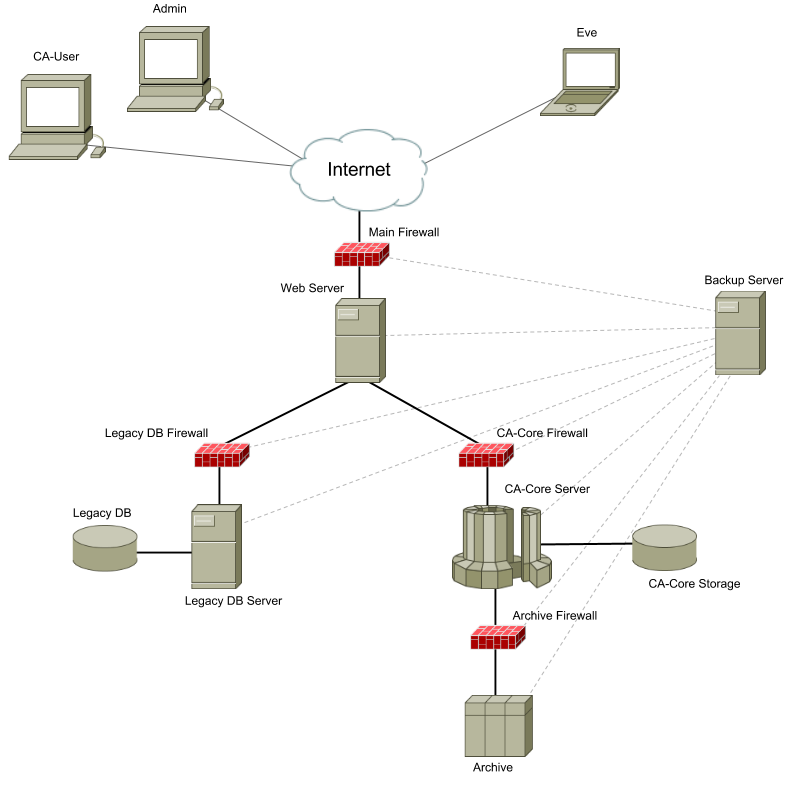
\includegraphics[scale=0.5]{network_diagram}
\caption{Network diagram}
\label{fig:network_diagram}
\end{figure}

The components (as depicted in figure~\ref{fig:network_diagram}) are as follows:

\begin{description}
\item[Main Firewall] A virtual machine running a software firewall in front of the whole internal network. It forwards TCP Packets on port 80 and port 443 to the web server, TCP packets on port 2211 to the web server, TCP packets on port 2220 and 2221 to the legacy db firewall, TCP packets on port 2230 and 2231 to the CA-Core firewall and TCP packets on port 2240 and 2241 to the archive firewall. It accepts TCP packets on port 2200 which is the port, the internal SSH daemon is bound to.

\item[Web Server] A virtual machine running \dots linux. It only accepts connections from the main firewall. The only running daemons on this server are a SSH daemon listening on port 2211 to administrate the server and a HTTP daemon listening on ports 80 and 443.

\item[Legacy DB Firewall] A virtual machine running a software firewall in front of the legacy database server. It forwards TCP connections on port 2221 and TCP connections from the web server on port 3306 to the legacy database. Additionally a SSH daemon is running on port 2220 to allow administrators to remotely administrate the firewall.

\item[Legacy DB Server] A virtual machine running \dots linux. It only accepts connections from the legacy db firewall. The only running daemons on this server are a SSH daemon accepting connections on port 2221 to administrate the server and a MySQL daemon on port 3306.

\item[CA-Core Firewall] A virtual machine running a software firewall in front of the CA-Core server. It forwards TCP connections on port 2231 and TCP connections from the web server on port 443 to the CA-Core. Additionally a SSH daemon is running on port 2230 to allow administrators to remotely administrate the firewall.

\item[CA-Core Server] A virtual machine running \dots linux. It only accepts connections from the CA-Core firewall. The only running daemons on this server are a SSH daemon listening on port 2231 to administrate the server and a not yet decided service listening on port 443.

\item[Archive Firewall] A virtual machine running a software firewall in front of the CA-Core server. It forwards TCP connections on port 2241 and TCP connections from the CA-Core on port 443 to the CA-Core Storage. Additionally a SSH daemon is running on port 2240 to allow administrators to remotely administrate the firewall.

\item[Archive Server] A virtual machine running \dots linux. It only accepts connections from the Archive firewall. The only running daemons on this server are a SSH daemon listening on port 2241 to administrate the server and a not yet decided service listening on port 443.

\item[Backup Server] A virtual maching running \dots linux. It accepts connections from the main firewall, the web server, the ca-core, the legacy db and the archive. A SSH daemon is listening on port 2250 to allow administrators to remotely administrate the server and allow the other servers to backup their configuration files and their log files.

\end{description}

\subsubsection{Applications}

\begin{description}

\item[User Web Interface] Web application, details not yet decided. Running on the web server.

\item[Administration Panel] Web application, details not yet decided. Running on the web server.

\item[Legacy DB] MySQL database with the legacy scheme. Running on the legacy DB server.

\item[CA-Core] Application using the OpenSSL library that provides basic interfaces to create new key pairs, sign existing key pairs and revoke certificates. Running on the CA-Core server.

\item[CA-Core Storage] A database that is used by the CA-Core to store certain data (details are t.b.d.). Running on the CA-Core server.

\item[Archive] Details not yet decided. Running on the archive server.

\item[Backup] Simple script that keeps multiple backups from the other servers (especially of all the configuration and log files). Running on the backup server.

\end{description}

\subsubsection{Data}

\begin{description}

\item[User Information] Basic information according to the schema of the legacy database. This includes the user's username, his first and last names, his email address and a hash of his password. This information is stored in the legacy database.

\item[Key Pairs] Consist of a private key and the according public key that the CA-Core can generate on request. They are stored permanently in the archive. It is important, that the CA-Core destroys his record of the private key as soon as possible.

\item[Certificates] A certificate that is signed by the CA-Core. It is also stored in the archive and additionally also in the CA-Storage (to allow certificates to be revoked).

\item[Certificate Revocation List] A list of certificates, that have been revoked by the CA-Core.

\item[Local Users] Credentials, that are used for system administration and communication between the components of the system.

\item[Configuration Files] Configuration files are binary files that configure configurable services like configuration configuring configurations.

\item[Log Files] Log files. Stored on the backup server.

\end{description}

\subsection{Interfaces}

Not yet standardized.

\subsubsection{Web Interface}

\subsubsection{Legacy DB Interface}

\subsubsection{CA-Core Interface}

\subsubsection{Archive Interface}


















\section{Risk Analysis and Security Measures}

\subsection{Information Assets}

\subsubsection{Physical Assets}
Each of the machines mentioned in the system description would be considered a physical asset and would have to be protected against violation of their physical integrity. Since we are working in a virtualized lab environment, we ignore the physical assets.
\subsubsection{Logical Assets}
\begin{description}
\item[Software] Includes operating systems and applications running on the physical assets. All software assets are configured and regularly updated by the system administrator.
\begin{description}
\item[Main Firewall] Running IPCop 2.0.6. Provides Firewall functionality, routing, NAT and VPN.  

\item[Web Server] Running \dots linux and \dots web server. 

\item[Second Firewall] Application level Firewall with like Zorp 3.4.6. 

\item[Legacy DB Server] Running \dots linux and MySQL 5.6.14. 

\item[CA-Core Server] Running \dots linux with OpenSSL 1.0.1e.

\item[Archive Firewall] Running IPCop 2.0.6. Provides Firewall functionality.

\item[Archive Server] Running \dots linux. 

\item[Backup Server] Running \dots linux. 

\end{description}
\item[Information/Data]
\begin{description}

\item[User Information] The value of username and password depends on the role of the user. Since all users can create and revoke certificates the information should be protected form unauthorized access. The same is true for changing the user information. User information of a CA admin enable slightly more functionality, but these are only for displaying information not changing.  The state space of this asset corresponds to the set of people who have access to the valid username/password combination. For displaying and changing authorization has to be given, for the password confidentiality is necessary.

\item[Key Pairs] A pair of private and public Key. The state space of this asset corresponds to the set of people who should have access both public and private key which is only the holder of the private key (The keys in the archive should not be accessible in general). Confidentiality of the private key has to be guaranteed all the time.

\item[Certificates] The certificate asset consists of the certificate and the person in the DB associated with the certificate. The state space of this asset corresponds to the set of people who should have access to the certificate, which should be everybody. The relation between the user information and the certificate is fixed, if one of both changes, the information becomes invalid.

\item[Certificate Revocation List] A list of certificates, that have been revoked, availability of this List is essential.

\item[Local User Information] Credentials, that are used for system administration and communication between the components of the system. This information is different for every system. The state space of this asset corresponds to the set of people who have access to the valid username/password combination which should only be one, the system administrator. Confidentiality of both username and password has to be ensured.

\item[Configuration Files] Describe the configuratons running on the software assets. Confidentiality of these files should be ensured.

\item[Log Files] Hold information about what happened on all the systems. For auditability the logs should not be writable by the system administrator and confidential for other entities.

\end{description}

\end{description}

\subsubsection{Persons}
At this point we list all the personnel that are involved in creating and revoking certificates as well as persons with access to information that gets produces in these processes.
\begin{description}
\item[User] Can create and revoke certificates and change user information. Is responsible for the confidentiality of his password and private keys on his own machine.
\item[CA Administrator] Same as for user only with a bit more read access.
\item[System Administrator]  Maintains the server infrastructure. Obviously the system administrator has access to all critical data on the system. Should not have access to the private keys on the CA-Core as well as in the archive.
\end{description}
\subsection{Threat Sources}

In this Lab we are using a virtual environment and therefore neglect the environmental thread sources.\\
\begin{description}
\item[Users:] Everybody who has an entry in the Database and crates and revokes certificates.

\item[Employees:] Which is namely just the system administrator and the CA administrator.

\item[Script Kiddies:] Since the systems considered are connected to the Internet, they are exposed to attacks by script kiddies.

\item[Skilled Hacker:] Skilled hackers are one of the biggest concerns to the system. They could try ton issue certificates in the name of the CA authority or gain access to private keys.

\item[Malware:] Of course malware must be taken into account. Although it is unlikely that directed malware will be used to attack the CA authority , there is still the problem of undirected malware.
\end{description}


\subsection{Risks and Countermeasures}

List all potential threats and the
  corresponding countermeasures. Estimate the risk based on 
  the information about the threat, the threat sources and the 
  corresponding countermeasure. For this purpose, use the following three
  tables.

%\subsubsection{Tools}

\begin{center}
\begin{tabular}{|l|p{10cm}|}
\hline
\multicolumn{2}{|c|}{\bf Impact} \\
\hline
Impact & Description \\
\hline
\hline
High   & \hspace*{20pt}
The event may result in loss of confidentiality of private keys or root access to the CA-Core which enables the issuing of certificates. \\
\hline
Medium & \hspace*{20pt}
The event may result in loss of availability of the service or loss of confidentiality of the user data but not private keys and root access on CA-Core. \\
\hline
Low   & \hspace*{20pt}
The event may result in an unwillingly revocation of certificates or temporarily unavailability of the service. \\
\hline
\end{tabular}
%
\vspace{5mm}
%
%\noindent \hspace*{10pt}


\begin{tabular}{|l|p{10cm}|}
\hline
\multicolumn{2}{|c|}{\bf Likelihood} \\
\hline
Likelihood & Description \\
\hline
\hline
High   & \hspace*{20pt}
The threat source is highly motivated and sufficiently capable of exploiting a given vulnerability in order to change the asset's state. The controls to prevent the vulnerability from being exploited are ineffective. \\
\hline
Medium & \hspace*{20pt}
The threat source is motivated and capable of exploiting a given vulnerability in order to change the asset's state, but controls are in place that may impede a successful exploit of the vulnerability. \\
\hline
Low   & \hspace*{20pt}
The threat source lacks motivation or capabilities to exploit a given vulnerability in order to change the asset's state. Another possibility that results in a low likelihood is the case where controls are in place that prevent (or at least significantly impede) the vulnerability from being exercised. \\
\hline
\end{tabular}
\end{center}

\vspace{5mm}

\begin{center}
\begin{tabular}{|l|c|c|c|}
\hline
\multicolumn{4}{|c|}{{\bf Risk Level}} \\
\hline
{{\bf Likelihood}} & \multicolumn{3}{c|}{{\bf Impact}} \\ %\cline{2-4}
     & Low & Medium & High \\  \hline
 High & Low & Medium & High  \\
\hline
 Medium & Low & Medium & Medium \\
\hline
 Low & Low & Low & Low \\
\hline
\end{tabular}
\end{center}

\subsubsection{{\it Evaluation Legacy DB \& User Information}}

%Evaluate the likelihood, impact and the resulting risk,  after implementation of the corresponding countermeasures.

\begin{footnotesize}
\begin{prettytablex}{p{0.1cm}p{2cm}p{5.5cm}XXX}
No. & Threat & Implemented/planned countermeasure(s) & L & I & Risk \\
\hline
1 & 
Alter information in the DB or DB itself without authorized access to do so
 & 
Prevent code injection in DB. Only open ports to webserver \& database that are needed for operation (firewall). 
  & {\it Medium} & {\it Medium} & {\it Medium} \\
\hline
2 & 
Read out or get access to user information and/or passwords
 & 
Prevent access to DB server. Encrypt passwords.
 & {\it Medium} & {\it High} & {\it Medium} \\
\hline
%2 & ... & ...& {\it ...} & {\it ...} & {\it ...} \\
%\hline
\end{prettytablex}
\end{footnotesize}



\subsubsection{{\it Evaluation Certification Revocation List}}

\begin{footnotesize}
\begin{prettytablex}{p{0.1cm}p{2cm}p{5.5cm}XXX}
No. & Threat & Implemented/planned countermeasure(s) & L & I & Risk \\
\hline
3 & 
Revoke certifications without holding the certificate
 & 
Ensure authorization before actions.
  & {\it Low} & {\it Low} & {\it Low} \\
\hline
\end{prettytablex}
\end{footnotesize}

\subsubsection{{\it Evaluation CA-Core Server \& Local User Information}}

\begin{footnotesize}
\begin{prettytablex}{p{0.1cm}p{2cm}p{5.5cm}XXX}
No. & Threat & Implemented/planned countermeasure(s) & L & I & Risk \\
\hline
4 & 
Issue certificates in the name of the CA
 & 
Limit access to machines via VPN and firewall \& ensure authorization before to get root privileges 
  & {\it Medium} & {\it High} & {\it Medium} \\
\hline
\end{prettytablex}
\end{footnotesize}

\subsubsection{{\it Evaluation Key Pairs a \& Archive}}

\begin{footnotesize}
\begin{prettytablex}{p{0.1cm}p{2cm}p{5.5cm}XXX}
No. & Threat & Implemented/planned countermeasure(s) & L & I & Risk \\
\hline
5 & 
Access to private key during transmission of certificate to user after issuing it
 & 
Encrypt communication between CA-Core and webserver as well as webserver and user
  & {\it Medium} & {\it High} & {\it Medium} \\
\hline
6 & 
Access to private key by accessing the CA-Core
 & 
Instantly delete private keys on CA-Core after issuing to user and archiving. Protect access to server
 & {\it Low} & {\it High} & {\it Low} \\
\hline
7 & 
Access private key by accessing and decrypting backup stored in archive
 & 
Protect access to archive, encrypt key backup and protect key for encryption 
  & {\it Low} & {\it High} & {\it Low} \\
\hline
\end{prettytablex}
\end{footnotesize}

\subsubsection{{\it Evaluation Local User Information \& all Servers}}

\begin{footnotesize}
\begin{prettytablex}{p{0.1cm}p{2cm}p{5.5cm}XXX}
No. & Threat & Implemented/planned countermeasure(s) & L & I & Risk \\
\hline
8 & 
Root access/login on every hardware other then the web server
 & 
Only allow access via SSH from within network (VPN), use different and strong authentication on every server
  & {\it Medium} & {\it High} & {\it Medium} \\
\hline
\end{prettytablex}
\end{footnotesize}

\subsubsection{{\it Evaluation all hardware \& software}}

\begin{footnotesize}
\begin{prettytablex}{p{0.1cm}p{2cm}p{5.5cm}XXX}
No. & Threat & Implemented/planned countermeasure(s) & L & I & Risk \\
\hline
9 & 
Denial of service
 & 
Not much, no confidentiality of key parts are at stake. Could try load balancing \& getting additional hardware/bandwidth
  & {\it Medium} & {\it Low} & {\it Low} \\
\hline
\end{prettytablex}
\end{footnotesize}



\subsubsection{Risk Acceptance}

%List all medium and high risks, according to the evaluation above. For each risk, propose additional countermeasures that could be implemented to further reduce the risks.

\begin{footnotesize}
\begin{prettytablex}{p{2cm}X}
No. of threat & Proposed countermeasure including expected impact  \\
\hline
1 & Allow only users to alter data when authenticated and operating on an encrypted connection. Don't allow altering the DB, just update the fields belonging to the user \\
\hline
2 & Enforce use of strong passwords \\
\hline
4 & Enforce strong passwords, implement two factor authentication for access to critical hardware/software. Don't let processes run with root privileges if not necessary  \\
\hline
5 & In addition to secure channel, decrypt public and private key on transmission \\
\hline
6 & Never write key to disk, encrypt and send to user and archive \\
\hline
7 & Enforce strong passwords, implement two factor authentication for access to critical hardware/software. \\
\hline
8 & Enforce strong passwords, implement two factor authentication for access to critical hardware/software \\
\hline
\end{prettytablex}
\end{footnotesize}

\end{document}
